\chapter{Classes natives}

À l'utilisation de l'interface native, le programmeur doit fréquemment conserver une référence à un espace mémoire ou une donnée C dans le code Nit. Traditionnellement, dans les autres interfaces, cet espace mémoire est opaque au langage de haut niveau et il y est représenté par un type général.


\section{Représentation des types C en Nit}

La figure~\ref{fig:hybride} présente quelque chose.


\begin{figure}[t]
\begin{center}
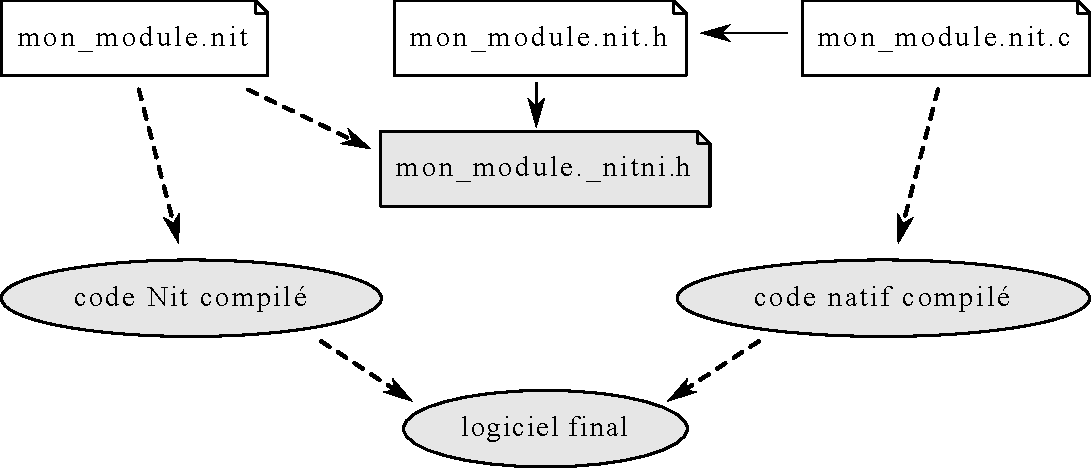
\includegraphics[width=4in]{figures/hybride}

\caption[Short name for the list of figures]{Real caption: Structure of JNI residing between the JVM and the native code.

The JNI is the interface for all JVM functionalities accessible from C. It exposes enough internals of the JVM offering a wide range of uses.}
\label{fig:hybride}
\end{center}
\end{figure}
